\documentclass[tikz,border=0pt]{standalone}
\usepackage{xcolor}
\usetikzlibrary{calc}
% Palette: Sam_Comm_final.png by eye, and the drones and raiders.
\definecolor{ink}{HTML}{3B2340}
\definecolor{sky}{HTML}{EFC46A}
\definecolor{skyhi}{HTML}{F5DA92}
\definecolor{skylow}{HTML}{E9B060}
\definecolor{cloud}{HTML}{F2D58A}
\definecolor{paper}{HTML}{FBEFD0}
\definecolor{cream}{HTML}{FFF6E0}
\definecolor{white}{HTML}{FFFFFF}
\definecolor{wallA}{HTML}{E88A73}
\definecolor{wallB}{HTML}{EE9F7E}
\definecolor{wallC}{HTML}{E47A7E}
\definecolor{wallD}{HTML}{F0B07E}
\definecolor{wallE}{HTML}{D9765F}
\definecolor{wallF}{HTML}{E99A8A}
\definecolor{greenA}{HTML}{8DBB7E}
\definecolor{greenB}{HTML}{6FA77A}
\definecolor{greenC}{HTML}{A9C97F}
\definecolor{greenD}{HTML}{5E9C6A}
\definecolor{greenE}{HTML}{4A8060}
\definecolor{sage}{HTML}{9DB98A}
\definecolor{sagedark}{HTML}{6F8F66}
\definecolor{sagelight}{HTML}{C2D6A6}
\definecolor{window}{HTML}{F6E7A0}
\definecolor{windark}{HTML}{8C5A64}
\definecolor{metal}{HTML}{8D9A93}
\definecolor{metaldark}{HTML}{5E6B66}
\definecolor{metallight}{HTML}{B9C4BC}
\definecolor{wood}{HTML}{B9835A}
\definecolor{wooddark}{HTML}{8C5A3C}
\definecolor{woodlight}{HTML}{D9A66F}
\definecolor{stone}{HTML}{E7C9A0}
\definecolor{stonedark}{HTML}{C9A47E}
\definecolor{concrete}{HTML}{D8C3A4}
\definecolor{concretedark}{HTML}{B8A084}
\definecolor{asphalt}{HTML}{8E7A86}
\definecolor{asphaltdark}{HTML}{6E5C68}
\definecolor{roadline}{HTML}{F6E7A0}
\definecolor{kerb}{HTML}{D8B48C}
\definecolor{red}{HTML}{E0483E}
\definecolor{redlight}{HTML}{F27A6A}
\definecolor{gold}{HTML}{FFB000}
\definecolor{goldlight}{HTML}{FFD54F}
\definecolor{teal}{HTML}{4FA3A0}
\definecolor{tealdark}{HTML}{3C8582}
\definecolor{magenta}{HTML}{FF2E88}
\definecolor{cyan}{HTML}{13CFE3}
\definecolor{violet}{HTML}{8A5BD6}
\definecolor{orange}{HTML}{F2803A}
\definecolor{pink}{HTML}{F48FB1}
\definecolor{glow}{HTML}{4FE6E0}
\definecolor{glowhi}{HTML}{C8FFF9}
\definecolor{hot}{HTML}{FF6A1A}
\definecolor{hothi}{HTML}{FFD07A}
\definecolor{armour}{HTML}{7E7A86}
\definecolor{armourdark}{HTML}{5A5466}
\definecolor{armourlight}{HTML}{A8A2B0}
\definecolor{wasp}{HTML}{E0A82E}
\definecolor{waspdark}{HTML}{B07E1A}
\definecolor{moth}{HTML}{F2E6C8}
\definecolor{mothdark}{HTML}{D2C09A}
\definecolor{hornet}{HTML}{3C8582}
\definecolor{hornetdark}{HTML}{2C6260}
\definecolor{warden}{HTML}{E47A7E}
\definecolor{wardendark}{HTML}{B85A62}
\definecolor{tick}{HTML}{8DBB7E}
\definecolor{tickdark}{HTML}{5E8A5A}
\definecolor{strider}{HTML}{D9765F}
\definecolor{striderdark}{HTML}{A8543F}
\definecolor{jacket}{HTML}{6FA77A}
\definecolor{jacketb}{HTML}{4FA3A0}
\definecolor{jacketc}{HTML}{E88A73}
\definecolor{jacketd}{HTML}{F0B07E}
\definecolor{skin}{HTML}{F2C49A}
\definecolor{skinb}{HTML}{C98C6A}
\definecolor{skinc}{HTML}{8C5A3C}
\definecolor{hair}{HTML}{3B2340}
\definecolor{goo}{HTML}{B6E35A}
\definecolor{goodark}{HTML}{7FB23A}
\newcommand{\Ink}{1.6pt}
\tikzset{inked/.style={draw=ink, line width=\Ink, line join=round, line cap=round}}
\begin{document}
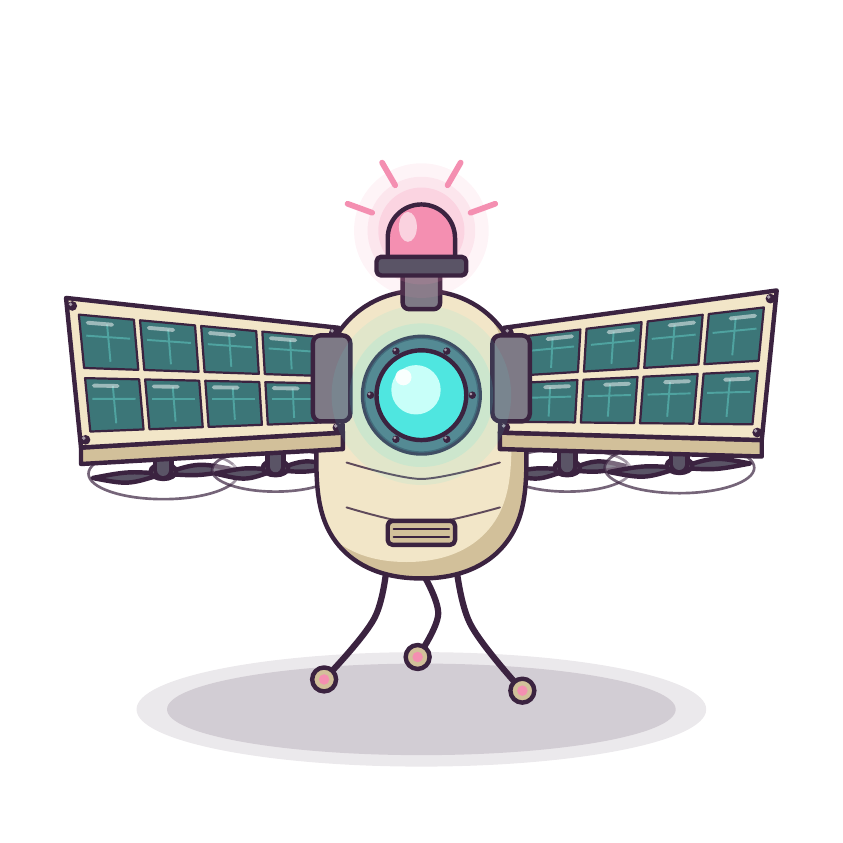
\begin{tikzpicture}
\clip (0,0) rectangle (10,10);
\begin{scope}[shift={(0.25,0.25)}, scale=0.95]
\fill[ink, opacity=0.10] (5,1.15) ellipse (3.808 and 0.765);
\fill[ink, opacity=0.14] (5,1.15) ellipse (3.4 and 0.612);
\filldraw[ink, line width=0.96pt, fill=white, fill opacity=0.32, draw opacity=0.7] (1.55,4.3) ellipse (1 and 0.34);
\fill[white, opacity=0.35] (1.55,4.3) ellipse (0.72 and 0.245);
\filldraw[inked,fill=armourdark] (1.55,4.3) .. controls (2.016,4.448) .. (2.495,4.357) .. controls (2.026,4.268) .. (1.55,4.3) -- cycle;
\filldraw[inked,fill=armourdark] (1.55,4.3) .. controls (1.084,4.152) .. (0.605,4.243) .. controls (1.074,4.332) .. (1.55,4.3) -- cycle;
\filldraw[inked,fill=metal] (1.55,4.33) ellipse (0.17 and 0.1);
\draw[ink, line width=7.525pt, line cap=round, line join=round] plot[smooth, tension=0.55] coordinates {(1.55,4.35) (1.55,4.65)};
\draw[armourdark, line width=4.325pt, line cap=round, line join=round] plot[smooth, tension=0.55] coordinates {(1.55,4.35) (1.55,4.65)};
\filldraw[ink, line width=0.96pt, fill=white, fill opacity=0.32, draw opacity=0.7] (3.05,4.35) ellipse (0.85 and 0.289);
\fill[white, opacity=0.35] (3.05,4.35) ellipse (0.612 and 0.208);
\filldraw[inked,fill=armourdark] (3.05,4.35) .. controls (3.445,4.494) .. (3.854,4.398) .. controls (3.455,4.314) .. (3.05,4.35) -- cycle;
\filldraw[inked,fill=armourdark] (3.05,4.35) .. controls (2.655,4.206) .. (2.246,4.302) .. controls (2.645,4.386) .. (3.05,4.35) -- cycle;
\filldraw[inked,fill=metal] (3.05,4.38) ellipse (0.17 and 0.1);
\draw[ink, line width=7.525pt, line cap=round, line join=round] plot[smooth, tension=0.55] coordinates {(3.05,4.4) (3.05,4.7)};
\draw[armourdark, line width=4.325pt, line cap=round, line join=round] plot[smooth, tension=0.55] coordinates {(3.05,4.4) (3.05,4.7)};
\filldraw[ink, line width=0.96pt, fill=white, fill opacity=0.32, draw opacity=0.7] (6.95,4.35) ellipse (0.85 and 0.289);
\fill[white, opacity=0.35] (6.95,4.35) ellipse (0.612 and 0.208);
\filldraw[inked,fill=armourdark] (6.95,4.35) .. controls (7.345,4.494) .. (7.754,4.398) .. controls (7.355,4.314) .. (6.95,4.35) -- cycle;
\filldraw[inked,fill=armourdark] (6.95,4.35) .. controls (6.555,4.206) .. (6.146,4.302) .. controls (6.545,4.386) .. (6.95,4.35) -- cycle;
\filldraw[inked,fill=metal] (6.95,4.38) ellipse (0.17 and 0.1);
\draw[ink, line width=7.525pt, line cap=round, line join=round] plot[smooth, tension=0.55] coordinates {(6.95,4.4) (6.95,4.7)};
\draw[armourdark, line width=4.325pt, line cap=round, line join=round] plot[smooth, tension=0.55] coordinates {(6.95,4.4) (6.95,4.7)};
\filldraw[ink, line width=0.96pt, fill=white, fill opacity=0.32, draw opacity=0.7] (8.45,4.38) ellipse (1 and 0.34);
\fill[white, opacity=0.35] (8.45,4.38) ellipse (0.72 and 0.245);
\filldraw[inked,fill=armourdark] (8.45,4.38) .. controls (8.916,4.528) .. (9.395,4.437) .. controls (8.926,4.348) .. (8.45,4.38) -- cycle;
\filldraw[inked,fill=armourdark] (8.45,4.38) .. controls (7.984,4.232) .. (7.505,4.323) .. controls (7.974,4.412) .. (8.45,4.38) -- cycle;
\filldraw[inked,fill=metal] (8.45,4.41) ellipse (0.17 and 0.1);
\draw[ink, line width=7.525pt, line cap=round, line join=round] plot[smooth, tension=0.55] coordinates {(8.45,4.43) (8.45,4.73)};
\draw[armourdark, line width=4.325pt, line cap=round, line join=round] plot[smooth, tension=0.55] coordinates {(8.45,4.43) (8.45,4.73)};
\draw[ink, line width=2.24pt, line cap=round, line join=round] plot[smooth, tension=0.6] coordinates {(4.55,3.2) (4.375,2.375) (3.7,1.55)};
\filldraw[inked,fill=mothdark] (3.7,1.55) circle (0.16);
\fill[pink] (3.7,1.55) circle (0.07);
\draw[ink, line width=2.24pt, line cap=round, line join=round] plot[smooth, tension=0.6] coordinates {(5.45,3.2) (5.65,2.3) (6.35,1.4)};
\filldraw[inked,fill=mothdark] (6.35,1.4) circle (0.16);
\fill[pink] (6.35,1.4) circle (0.07);
\draw[ink, line width=2.24pt, line cap=round, line join=round] plot[smooth, tension=0.6] coordinates {(5,3) (5.225,2.425) (4.95,1.85)};
\filldraw[inked,fill=mothdark] (4.95,1.85) circle (0.16);
\fill[pink] (4.95,1.85) circle (0.07);
\fill[mothdark] plot[smooth cycle, tension=0.7] coordinates {(5,2.9) (6.15,3.4) (6.4,4.8) (6.1,6.2) (5,6.75) (3.9,6.2) (3.6,4.8) (3.85,3.4)};
\begin{scope}\clip plot[smooth cycle, tension=0.7] coordinates {(5,2.9) (6.15,3.4) (6.4,4.8) (6.1,6.2) (5,6.75) (3.9,6.2) (3.6,4.8) (3.85,3.4)};
\begin{scope}[shift={(-0.2,0.22)}]\fill[moth] plot[smooth cycle, tension=0.7] coordinates {(5,2.9) (6.15,3.4) (6.4,4.8) (6.1,6.2) (5,6.75) (3.9,6.2) (3.6,4.8) (3.85,3.4)};\end{scope}
\end{scope}
\draw[inked] plot[smooth cycle, tension=0.7] coordinates {(5,2.9) (6.15,3.4) (6.4,4.8) (6.1,6.2) (5,6.75) (3.9,6.2) (3.6,4.8) (3.85,3.4)};
\draw[ink, line width=0.7pt, line cap=round, line join=round, opacity=0.8] plot[smooth, tension=0.5] coordinates {(4,3.85) (5,3.63) (6.05,3.85)};
\draw[ink, line width=0.7pt, line cap=round, line join=round, opacity=0.8] plot[smooth, tension=0.5] coordinates {(4,4.45) (5,4.23) (6.05,4.45)};
\filldraw[inked,fill=mothdark,rounded corners=0.06cm] (4.55,3.35) rectangle (5.45,3.67);
\draw[ink, line width=0.8pt, line cap=round] (4.63,3.457) -- (5.37,3.457);
\draw[ink, line width=0.8pt, line cap=round] (4.63,3.563) -- (5.37,3.563);
\filldraw[inked,fill=mothdark] (0.45,4.65) -- (3.95,4.85) -- (3.95,4.63) -- (0.45,4.43) -- cycle;
\filldraw[inked,fill=moth] (0.25,6.65) -- (3.9,6.25) -- (3.95,4.85) -- (0.45,4.65) -- cycle;
\filldraw[inked,fill=tealdark!85!ink,line width=0.8pt] (0.421,6.427) -- (1.157,6.359) -- (1.216,5.689) -- (0.491,5.714) -- cycle;
\draw[teal, line width=0.7pt] (0.52,6.146) -- (1.107,6.105);
\draw[teal, line width=0.7pt] (0.798,6.297) -- (0.844,5.797);
\draw[white, opacity=0.5, line width=1.4pt, line cap=round] (0.539,6.319) -- (0.866,6.292);
\filldraw[inked,fill=tealdark!85!ink,line width=0.8pt] (0.504,5.578) -- (1.227,5.562) -- (1.286,4.892) -- (0.574,4.864) -- cycle;
\draw[teal, line width=0.7pt] (0.602,5.301) -- (1.179,5.302);
\draw[teal, line width=0.7pt] (0.875,5.474) -- (0.921,4.974);
\draw[white, opacity=0.5, line width=1.4pt, line cap=round] (0.621,5.478) -- (0.941,5.473);
\filldraw[inked,fill=tealdark!85!ink,line width=0.8pt] (1.239,6.351) -- (1.974,6.283) -- (2.021,5.662) -- (1.296,5.687) -- cycle;
\draw[teal, line width=0.7pt] (1.333,6.089) -- (1.92,6.048);
\draw[teal, line width=0.7pt] (1.614,6.228) -- (1.652,5.763);
\draw[white, opacity=0.5, line width=1.4pt, line cap=round] (1.355,6.25) -- (1.682,6.222);
\filldraw[inked,fill=tealdark!85!ink,line width=0.8pt] (1.307,5.56) -- (2.03,5.544) -- (2.077,4.923) -- (1.365,4.895) -- cycle;
\draw[teal, line width=0.7pt] (1.401,5.303) -- (1.977,5.303);
\draw[teal, line width=0.7pt] (1.676,5.463) -- (1.714,4.998);
\draw[white, opacity=0.5, line width=1.4pt, line cap=round] (1.422,5.467) -- (1.743,5.462);
\filldraw[inked,fill=tealdark!85!ink,line width=0.8pt] (2.056,6.275) -- (2.792,6.207) -- (2.827,5.635) -- (2.102,5.66) -- cycle;
\draw[teal, line width=0.7pt] (2.146,6.032) -- (2.733,5.99);
\draw[teal, line width=0.7pt] (2.43,6.159) -- (2.459,5.73);
\draw[white, opacity=0.5, line width=1.4pt, line cap=round] (2.171,6.181) -- (2.498,6.153);
\filldraw[inked,fill=tealdark!85!ink,line width=0.8pt] (2.111,5.542) -- (2.833,5.526) -- (2.868,4.954) -- (2.156,4.926) -- cycle;
\draw[teal, line width=0.7pt] (2.199,5.304) -- (2.776,5.304);
\draw[teal, line width=0.7pt] (2.478,5.452) -- (2.507,5.022);
\draw[white, opacity=0.5, line width=1.4pt, line cap=round] (2.224,5.455) -- (2.544,5.451);
\filldraw[inked,fill=tealdark!85!ink,line width=0.8pt] (2.874,6.2) -- (3.61,6.131) -- (3.632,5.608) -- (2.907,5.632) -- cycle;
\draw[teal, line width=0.7pt] (2.959,5.975) -- (3.546,5.933);
\draw[teal, line width=0.7pt] (3.246,6.09) -- (3.266,5.696);
\draw[white, opacity=0.5, line width=1.4pt, line cap=round] (2.987,6.112) -- (3.314,6.084);
\filldraw[inked,fill=tealdark!85!ink,line width=0.8pt] (2.914,5.524) -- (3.637,5.508) -- (3.659,4.985) -- (2.947,4.957) -- cycle;
\draw[teal, line width=0.7pt] (2.998,5.305) -- (3.574,5.305);
\draw[teal, line width=0.7pt] (3.279,5.441) -- (3.299,5.047);
\draw[white, opacity=0.5, line width=1.4pt, line cap=round] (3.025,5.444) -- (3.346,5.44);
\fill[ink] (0.333,6.543) circle (0.065);
\fill[white, opacity=0.55] (0.31,6.565) circle (0.026);
\fill[ink] (0.51,4.753) circle (0.065);
\fill[white, opacity=0.55] (0.487,4.776) circle (0.026);
\fill[ink] (3.83,6.187) circle (0.065);
\fill[white, opacity=0.55] (3.807,6.21) circle (0.026);
\fill[ink] (3.877,4.917) circle (0.065);
\fill[white, opacity=0.55] (3.855,4.939) circle (0.026);
\filldraw[inked,fill=armour,rounded corners=0.1cm] (3.55,5) rectangle (4.05,6.15);
\filldraw[inked,fill=mothdark] (9.55,4.75) -- (6.05,4.85) -- (6.05,4.63) -- (9.55,4.53) -- cycle;
\filldraw[inked,fill=moth] (9.75,6.75) -- (6.1,6.25) -- (6.05,4.85) -- (9.55,4.75) -- cycle;
\filldraw[inked,fill=tealdark!85!ink,line width=0.8pt] (9.579,6.523) -- (8.843,6.435) -- (8.784,5.765) -- (9.509,5.81) -- cycle;
\draw[teal, line width=0.7pt] (9.48,6.24) -- (8.893,6.182);
\draw[teal, line width=0.7pt] (9.202,6.383) -- (9.156,5.883);
\draw[white, opacity=0.5, line width=1.4pt, line cap=round] (9.461,6.412) -- (9.134,6.376);
\filldraw[inked,fill=tealdark!85!ink,line width=0.8pt] (9.496,5.674) -- (8.773,5.637) -- (8.714,4.968) -- (9.426,4.96) -- cycle;
\draw[teal, line width=0.7pt] (9.398,5.395) -- (8.821,5.38);
\draw[teal, line width=0.7pt] (9.125,5.56) -- (9.079,5.06);
\draw[white, opacity=0.5, line width=1.4pt, line cap=round] (9.379,5.571) -- (9.059,5.557);
\filldraw[inked,fill=tealdark!85!ink,line width=0.8pt] (8.761,6.425) -- (8.026,6.336) -- (7.979,5.715) -- (8.704,5.76) -- cycle;
\draw[teal, line width=0.7pt] (8.667,6.16) -- (8.08,6.103);
\draw[teal, line width=0.7pt] (8.386,6.291) -- (8.348,5.827);
\draw[white, opacity=0.5, line width=1.4pt, line cap=round] (8.645,6.321) -- (8.318,6.284);
\filldraw[inked,fill=tealdark!85!ink,line width=0.8pt] (8.693,5.633) -- (7.97,5.597) -- (7.923,4.976) -- (8.635,4.969) -- cycle;
\draw[teal, line width=0.7pt] (8.599,5.374) -- (8.023,5.358);
\draw[teal, line width=0.7pt] (8.324,5.526) -- (8.286,5.062);
\draw[white, opacity=0.5, line width=1.4pt, line cap=round] (8.578,5.537) -- (8.257,5.524);
\filldraw[inked,fill=tealdark!85!ink,line width=0.8pt] (7.944,6.326) -- (7.208,6.238) -- (7.173,5.666) -- (7.898,5.71) -- cycle;
\draw[teal, line width=0.7pt] (7.854,6.081) -- (7.267,6.023);
\draw[teal, line width=0.7pt] (7.57,6.2) -- (7.541,5.77);
\draw[white, opacity=0.5, line width=1.4pt, line cap=round] (7.829,6.229) -- (7.502,6.192);
\filldraw[inked,fill=tealdark!85!ink,line width=0.8pt] (7.889,5.593) -- (7.167,5.557) -- (7.132,4.985) -- (7.844,4.977) -- cycle;
\draw[teal, line width=0.7pt] (7.801,5.352) -- (7.224,5.337);
\draw[teal, line width=0.7pt] (7.522,5.493) -- (7.493,5.063);
\draw[white, opacity=0.5, line width=1.4pt, line cap=round] (7.776,5.503) -- (7.456,5.49);
\filldraw[inked,fill=tealdark!85!ink,line width=0.8pt] (7.126,6.228) -- (6.39,6.139) -- (6.368,5.616) -- (7.093,5.661) -- cycle;
\draw[teal, line width=0.7pt] (7.041,6.001) -- (6.454,5.944);
\draw[teal, line width=0.7pt] (6.754,6.108) -- (6.734,5.714);
\draw[white, opacity=0.5, line width=1.4pt, line cap=round] (7.013,6.137) -- (6.686,6.101);
\filldraw[inked,fill=tealdark!85!ink,line width=0.8pt] (7.086,5.553) -- (6.363,5.516) -- (6.341,4.993) -- (7.053,4.986) -- cycle;
\draw[teal, line width=0.7pt] (7.002,5.331) -- (6.426,5.315);
\draw[teal, line width=0.7pt] (6.721,5.459) -- (6.701,5.065);
\draw[white, opacity=0.5, line width=1.4pt, line cap=round] (6.975,5.47) -- (6.654,5.456);
\fill[ink] (9.667,6.641) circle (0.065);
\fill[white, opacity=0.55] (9.644,6.663) circle (0.026);
\fill[ink] (9.49,4.851) circle (0.065);
\fill[white, opacity=0.55] (9.467,4.874) circle (0.026);
\fill[ink] (6.17,6.189) circle (0.065);
\fill[white, opacity=0.55] (6.148,6.212) circle (0.026);
\fill[ink] (6.123,4.919) circle (0.065);
\fill[white, opacity=0.55] (6.1,4.941) circle (0.026);
\filldraw[inked,fill=armour,rounded corners=0.1cm] (5.95,5) rectangle (6.45,6.15);
\filldraw[inked,fill=armourdark] (5,5.35) circle (0.78);
\fill[glow, opacity=0.1] (5,5.35) ellipse (1.2 and 1.2);
\fill[glow, opacity=0.14] (5,5.35) ellipse (0.96 and 0.96);
\fill[glow, opacity=0.2] (5,5.35) ellipse (0.768 and 0.768);
\filldraw[inked,fill=glow] (5,5.35) ellipse (0.6 and 0.6);
\fill[glowhi]  (4.928,5.422) ellipse (0.33 and 0.33);
\fill[white, opacity=0.9] (4.76,5.59) circle (0.108);
\fill[ink] (5.68,5.35) circle (0.05);
\fill[white, opacity=0.55] (5.662,5.367) circle (0.02);
\fill[ink] (5.34,5.939) circle (0.05);
\fill[white, opacity=0.55] (5.322,5.956) circle (0.02);
\fill[ink] (4.66,5.939) circle (0.05);
\fill[white, opacity=0.55] (4.643,5.956) circle (0.02);
\fill[ink] (4.32,5.35) circle (0.05);
\fill[white, opacity=0.55] (4.303,5.367) circle (0.02);
\fill[ink] (4.66,4.761) circle (0.05);
\fill[white, opacity=0.55] (4.643,4.779) circle (0.02);
\fill[ink] (5.34,4.761) circle (0.05);
\fill[white, opacity=0.55] (5.322,4.779) circle (0.02);
\filldraw[inked,fill=armour,rounded corners=0.08cm] (4.75,6.5) rectangle (5.25,7.15);
\fill[pink, opacity=0.1] (5,7.55) ellipse (0.9 and 0.9);
\fill[pink, opacity=0.14] (5,7.55) ellipse (0.72 and 0.72);
\fill[pink, opacity=0.2] (5,7.55) ellipse (0.576 and 0.576);
\draw[pink, line width=2.08pt, line cap=round] (5.658,7.789) -- (5.987,7.909);
\draw[pink, line width=2.08pt, line cap=round] (5.35,8.156) -- (5.525,8.459);
\draw[pink, line width=2.08pt, line cap=round] (4.65,8.156) -- (4.475,8.459);
\draw[pink, line width=2.08pt, line cap=round] (4.342,7.789) -- (4.013,7.909);
\filldraw[inked, fill=pink] (4.55,7.15) -- (4.55,7.45) arc[start angle=180, end angle=0, radius=0.45] -- (5.45,7.15) -- cycle;
\fill[white, opacity=0.6] (4.82,7.6) ellipse (0.12 and 0.2);
\filldraw[inked,fill=armourdark,rounded corners=0.06cm] (4.4,6.95) rectangle (5.6,7.2);
\end{scope}
\end{tikzpicture}
\end{document}
